\chapter{KIẾN TRÚC HỆ THỐNG VÀ THIẾT KẾ DỮ LIỆU}
\label{ch:architecture}

\section{Kiến trúc Kỹ thuật Tổng thể (System Architecture)}
Hệ thống \textbf{Domanage} được xây dựng theo mô hình kiến trúc Single Page Application (SPA) hiện đại kết hợp với tầng dịch vụ RESTful API được mô phỏng linh hoạt, phân tách rõ ràng giữa tầng hiển thị (Presentation Layer), tầng xử lý nghiệp vụ (Business Logic Layer) và tầng lưu trữ dữ liệu (Data Layer).

\begin{figure}[htbp]
\centering
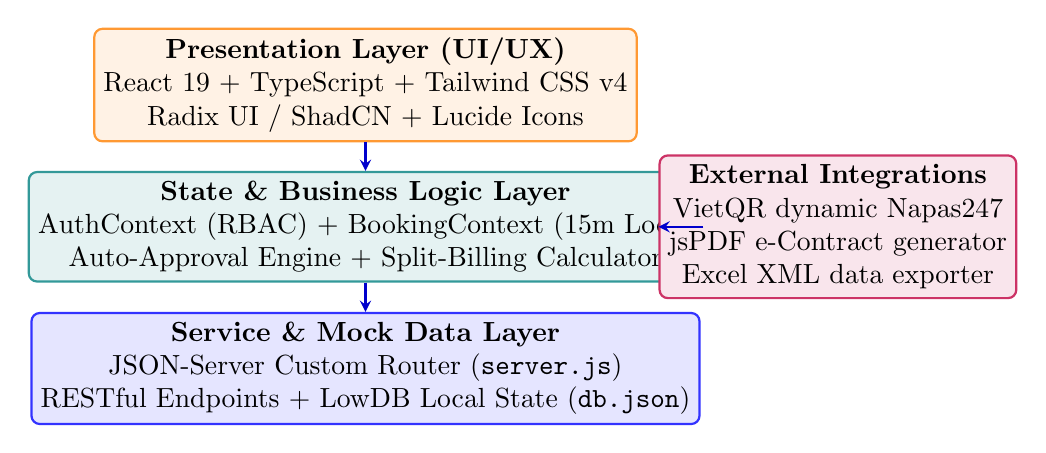
\begin{tikzpicture}[
    box/.style={rectangle, draw=blue!70!black, fill=blue!5, rounded corners=3pt, thick, align=center, minimum height=1cm},
    layer/.style={rectangle, draw=gray!60, fill=gray!5, dashed, rounded corners=6pt, inner sep=8pt},
    arrow/.style={->, >=stealth, thick, draw=blue!80!black}
]

% Client Layer
\node[box, fill=orange!10, draw=orange!80] (ui) at (0, 4) {\textbf{Presentation Layer (UI/UX)}\\React 19 + TypeScript + Tailwind CSS v4\\Radix UI / ShadCN + Lucide Icons};

% State & Context Layer
\node[box, fill=teal!10, draw=teal!80] (state) at (0, 2.2) {\textbf{State \& Business Logic Layer}\\AuthContext (RBAC) + BookingContext (15m Lock)\\Auto-Approval Engine + Split-Billing Calculator};

% API & Storage Layer
\node[box, fill=blue!10, draw=blue!80] (api) at (0, 0.4) {\textbf{Service \& Mock Data Layer}\\JSON-Server Custom Router (\texttt{server.js})\\RESTful Endpoints + LowDB Local State (\texttt{db.json})};

% External Services
\node[box, fill=purple!10, draw=purple!80] (ext) at (6, 2.2) {\textbf{External Integrations}\\VietQR dynamic Napas247\\jsPDF e-Contract generator\\Excel XML data exporter};

% Arrows
\draw[arrow] (ui) -- (state);
\draw[arrow] (state) -- (api);
\draw[arrow] (state) -- (ext);

\end{tikzpicture}
\caption{Sơ đồ phân tầng kiến trúc phần mềm hệ thống Domanage}
\label{fig:architecture_layers}
\end{figure}

\subsection{Tech Stack chi tiết}
\begin{itemize}
    \item \textbf{Frontend Framework:} React 19 kết hợp cùng TypeScript nghiêm ngặt (Strict Type Safety), mang lại hiệu năng cao và loại trừ lỗi runtime trong quá trình phát triển.
    \item \textbf{Styling \& Component Library:} Tailwind CSS v4 với kiến trúc CSS-first mới nhất, kết hợp các primitives không kiểu dáng từ Radix UI và bộ icon hiện đại Lucide React.
    \item \textbf{Routing \& Phân quyền:} \texttt{react-router-dom} (v7) kết hợp Component bậc cao \texttt{ProtectedRoute} để điều hướng tự động và kiểm soát quyền truy cập theo vai trò.
    \item \textbf{Báo cáo \& Xuất tệp:} \texttt{jspdf} tạo hợp đồng lưu trú điện tử tại máy khách, bộ công cụ tự tạo mã hóa XML xuất báo cáo danh sách tạm trú và công nợ sang định dạng bảng tính Microsoft Excel (\texttt{.xlsx}).
    \item \textbf{Biểu đồ phân tích:} Thư viện biểu đồ trực quan hóa dữ liệu tỷ lệ lấp đầy phòng (Occupancy Donut Chart) và xu hướng doanh thu (Revenue Trend Chart).
\end{itemize}

\section{Mô hình Không gian Phân cấp 1:4:6 (Spatial Topology)}
Một trong những đột phá sáng tạo của dự án là mô hình tổ chức không gian ký túc xá theo tỷ lệ \textbf{1:4:6}, phản ánh chân thực thiết kế phòng tiêu chuẩn tại Đại học FPT:
\begin{itemize}
    \item \textbf{Cấp 1 -- Tòa nhà (Building):} Đại diện cho một khối nhà ký túc xá (ví dụ: Tòa A -- Ký túc xá Nam, Tòa B -- Ký túc xá Nữ).
    \item \textbf{Cấp 2 -- Tầng lầu (Floor):} Mỗi tòa gồm 5 tầng lầu.
    \item \textbf{Cấp 3 -- Phòng ở (Room):} Mỗi tầng bố trí 4 phòng lớn (ví dụ: A101, A102, A103, A104).
    \item \textbf{Cấp 4 -- Buồng sinh hoạt (Compartment):} Mỗi phòng lớn được ngăn thành \textbf{4 buồng cá nhân} riêng biệt, định danh là \textbf{A, B, C, D}.
    \begin{itemize}
        \item \textit{Buồng A (Window Bay):} Hướng ban công/cửa sổ, đón ánh sáng tự nhiên.
        \item \textit{Buồng B (Balcony Wing):} Hướng đón gió mát, gần lối đi nội bộ.
        \item \textit{Buồng C (Study Corner):} Góc học tập yên tĩnh, thoáng đãng.
        \item \textit{Buồng D (Inner Suite):} Không gian ấm cúng, riêng tư tối đa.
    \end{itemize}
    \item \textbf{Cấp 5 -- Giường ngủ (Bed):} Mỗi buồng bao gồm \textbf{6 giường} (tương đương 3 giường tầng: Giường tầng dưới \textit{Lower} và Giường tầng trên \textit{Upper}), được đánh số từ \texttt{G01} đến \texttt{G06}.
\end{itemize}

Như vậy, mỗi phòng lớn có sức chứa tiêu chuẩn là $4 \times 6 = 24$ sinh viên. Toàn bộ mã giường trong hệ thống được chuẩn hóa theo quy tắc chuỗi ký tự bất biến:
\begin{center}
    \texttt{[Mã\_Phòng]-[Mã\_Buồng]-[Mã\_Giường]} $\quad\Longrightarrow\quad$ \textbf{\texttt{A205-B-G03}}
\end{center}

\section{Thiết kế Cơ sở Dữ liệu (Database Schema 12 Thực thể)}
Cơ sở dữ liệu được thiết kế đạt chuẩn chuẩn hóa bậc 3 (3NF) gồm 12 bảng thực thể chính. Chi tiết các thực thể được trình bày trong Bảng~\ref{tab:database_schema}.

\begin{table}[htbp]
\centering
\caption{Bảng từ điển dữ liệu 12 thực thể chính của hệ thống Domanage}
\label{tab:database_schema}
\small
\begin{tabularx}{\textwidth}{|l|l|X|}
\hline
\rowcolor{blue!10}
\textbf{Tên Bảng (Entity)} & \textbf{Khóa chính} & \textbf{Các thuộc tính chính và Mô tả} \\ \hline
\texttt{users} & \texttt{id} & \texttt{mssv}, \texttt{email}, \texttt{name}, \texttt{gender}, \texttt{role}, \texttt{status}, \texttt{previousDebt}, \texttt{isSuspended}, \texttt{disciplinePoints} (thang 100). \\ \hline
\texttt{buildings} & \texttt{id} & \texttt{name}, \texttt{genderType} (MALE/FEMALE), \texttt{totalFloors}. \\ \hline
\texttt{floors} & \texttt{id} & \texttt{buildingId} (FK), \texttt{level} (1--5). \\ \hline
\texttt{rooms} & \texttt{id} & \texttt{floorId} (FK), \texttt{name} (A101--A504), \texttt{status}. \\ \hline
\texttt{compartments} & \texttt{id} & \texttt{roomId} (FK), \texttt{name} (A, B, C, D), \texttt{title}, \texttt{zone}. \\ \hline
\texttt{beds} & \texttt{id} & \texttt{compartmentId} (FK), \texttt{slot} (G01--G06), \texttt{fullCode}, \texttt{tier} (upper/lower), \texttt{status} (available, holding, occupied, maintenance), \texttt{price}. \\ \hline
\texttt{bookings} & \texttt{id} & \texttt{userId} (FK), \texttt{bedId} (FK), \texttt{status} (PENDING, PAID, APPROVED, CANCELLED), \texttt{holdingExpiresAt}. \\ \hline
\texttt{contracts} & \texttt{id} & \texttt{bookingId} (FK), \texttt{userId} (FK), \texttt{bedCode}, \texttt{status} (ACTIVE, TERMINATED), \texttt{validFrom}, \texttt{validTo}. \\ \hline
\texttt{utilities} & \texttt{id} & \texttt{roomId} (FK), \texttt{month}, \texttt{elecOld}, \texttt{elecNew}, \texttt{waterOld}, \texttt{waterNew}, \texttt{elecPhotoUrl}, \texttt{waterPhotoUrl}, \texttt{status}. \\ \hline
\texttt{bills} & \texttt{id} & \texttt{utilityId} (FK), \texttt{userId} (FK), \texttt{amountTotal}, \texttt{status} (UNPAID, PAID), \texttt{qrCodeRef}, \texttt{dueDate}. \\ \hline
\texttt{maintenance\_tickets} & \texttt{id} & \texttt{userId} (FK), \texttt{scope} (ROOM/COMPARTMENT), \texttt{category}, \texttt{urgency}, \texttt{status}, \texttt{technicianId}, \texttt{rating}. \\ \hline
\texttt{gate\_passes} & \texttt{id} & \texttt{userId} (FK), \texttt{curfewDate}, \texttt{reason}, \texttt{expectedReturn}, \texttt{actualReturn}, \texttt{status} (PENDING, APPROVED, VIOLATED). \\ \hline
\end{tabularx}
\end{table}

\section{Vòng đời Trạng thái Giường (Bed State Machine)}
Mỗi vị trí giường ngủ trong hệ thống vận hành theo một máy trạng thái hữu hạn nghiêm ngặt nhằm giải quyết triệt để tình trạng xung đột đặt phòng đồng thời (Concurrency Race Conditions) như minh họa trong Hình~\ref{fig:bed_state_machine}.

\begin{figure}[htbp]
\centering
\begin{tikzpicture}[
    state/.style={circle, draw=blue!80, fill=blue!10, thick, minimum size=1.8cm, align=center, font=\footnotesize\bfseries},
    arrow/.style={->, >=stealth, thick}
]

\node[state, fill=green!15, draw=green!70!black] (avail) at (0, 0) {AVAILABLE\\(Còn trống)};
\node[state, fill=orange!20, draw=orange!80!black] (hold) at (4.5, 0) {HOLDING\\(Khóa 15m)};
\node[state, fill=gray!25, draw=gray!70!black] (occ) at (9, 0) {OCCUPIED\\(Đã ở)};
\node[state, fill=red!15, draw=red!70!black] (maint) at (4.5, -3) {MAINTENANCE\\(Bảo trì)};

\draw[arrow, draw=blue!80!black] (avail) -- node[above, font=\footnotesize] {Click chọn giường} (hold);
\draw[arrow, draw=green!70!black] (hold) -- node[above, font=\footnotesize] {Auto-Approved} (occ);
\draw[arrow, draw=red!70!black, dashed] (hold) to[bend left=30] node[below, font=\footnotesize] {Hết 900s hoặc Hủy} (avail);
\draw[arrow, draw=gray!80!black] (occ) to[bend right=45] node[above, font=\footnotesize] {Check-out trả phòng} (avail);
\draw[arrow, draw=purple!80!black] (avail) -- node[left, font=\footnotesize] {Phát hiện hỏng} (maint);
\draw[arrow, draw=purple!80!black] (maint) -- node[right, font=\footnotesize] {Nghiệm thu sửa xong} (avail);

\end{tikzpicture}
\caption{Sơ đồ chuyển đổi trạng thái của vị trí giường trong hệ thống}
\label{fig:bed_state_machine}
\end{figure}

